%**************************************************************
\subsubsection{Package it.tecsen.smacs.viewmodel}
\label{subsubsec:it-tecsen-smacs-viewmodel}

\begin{figure}[!h]
  \centering 
  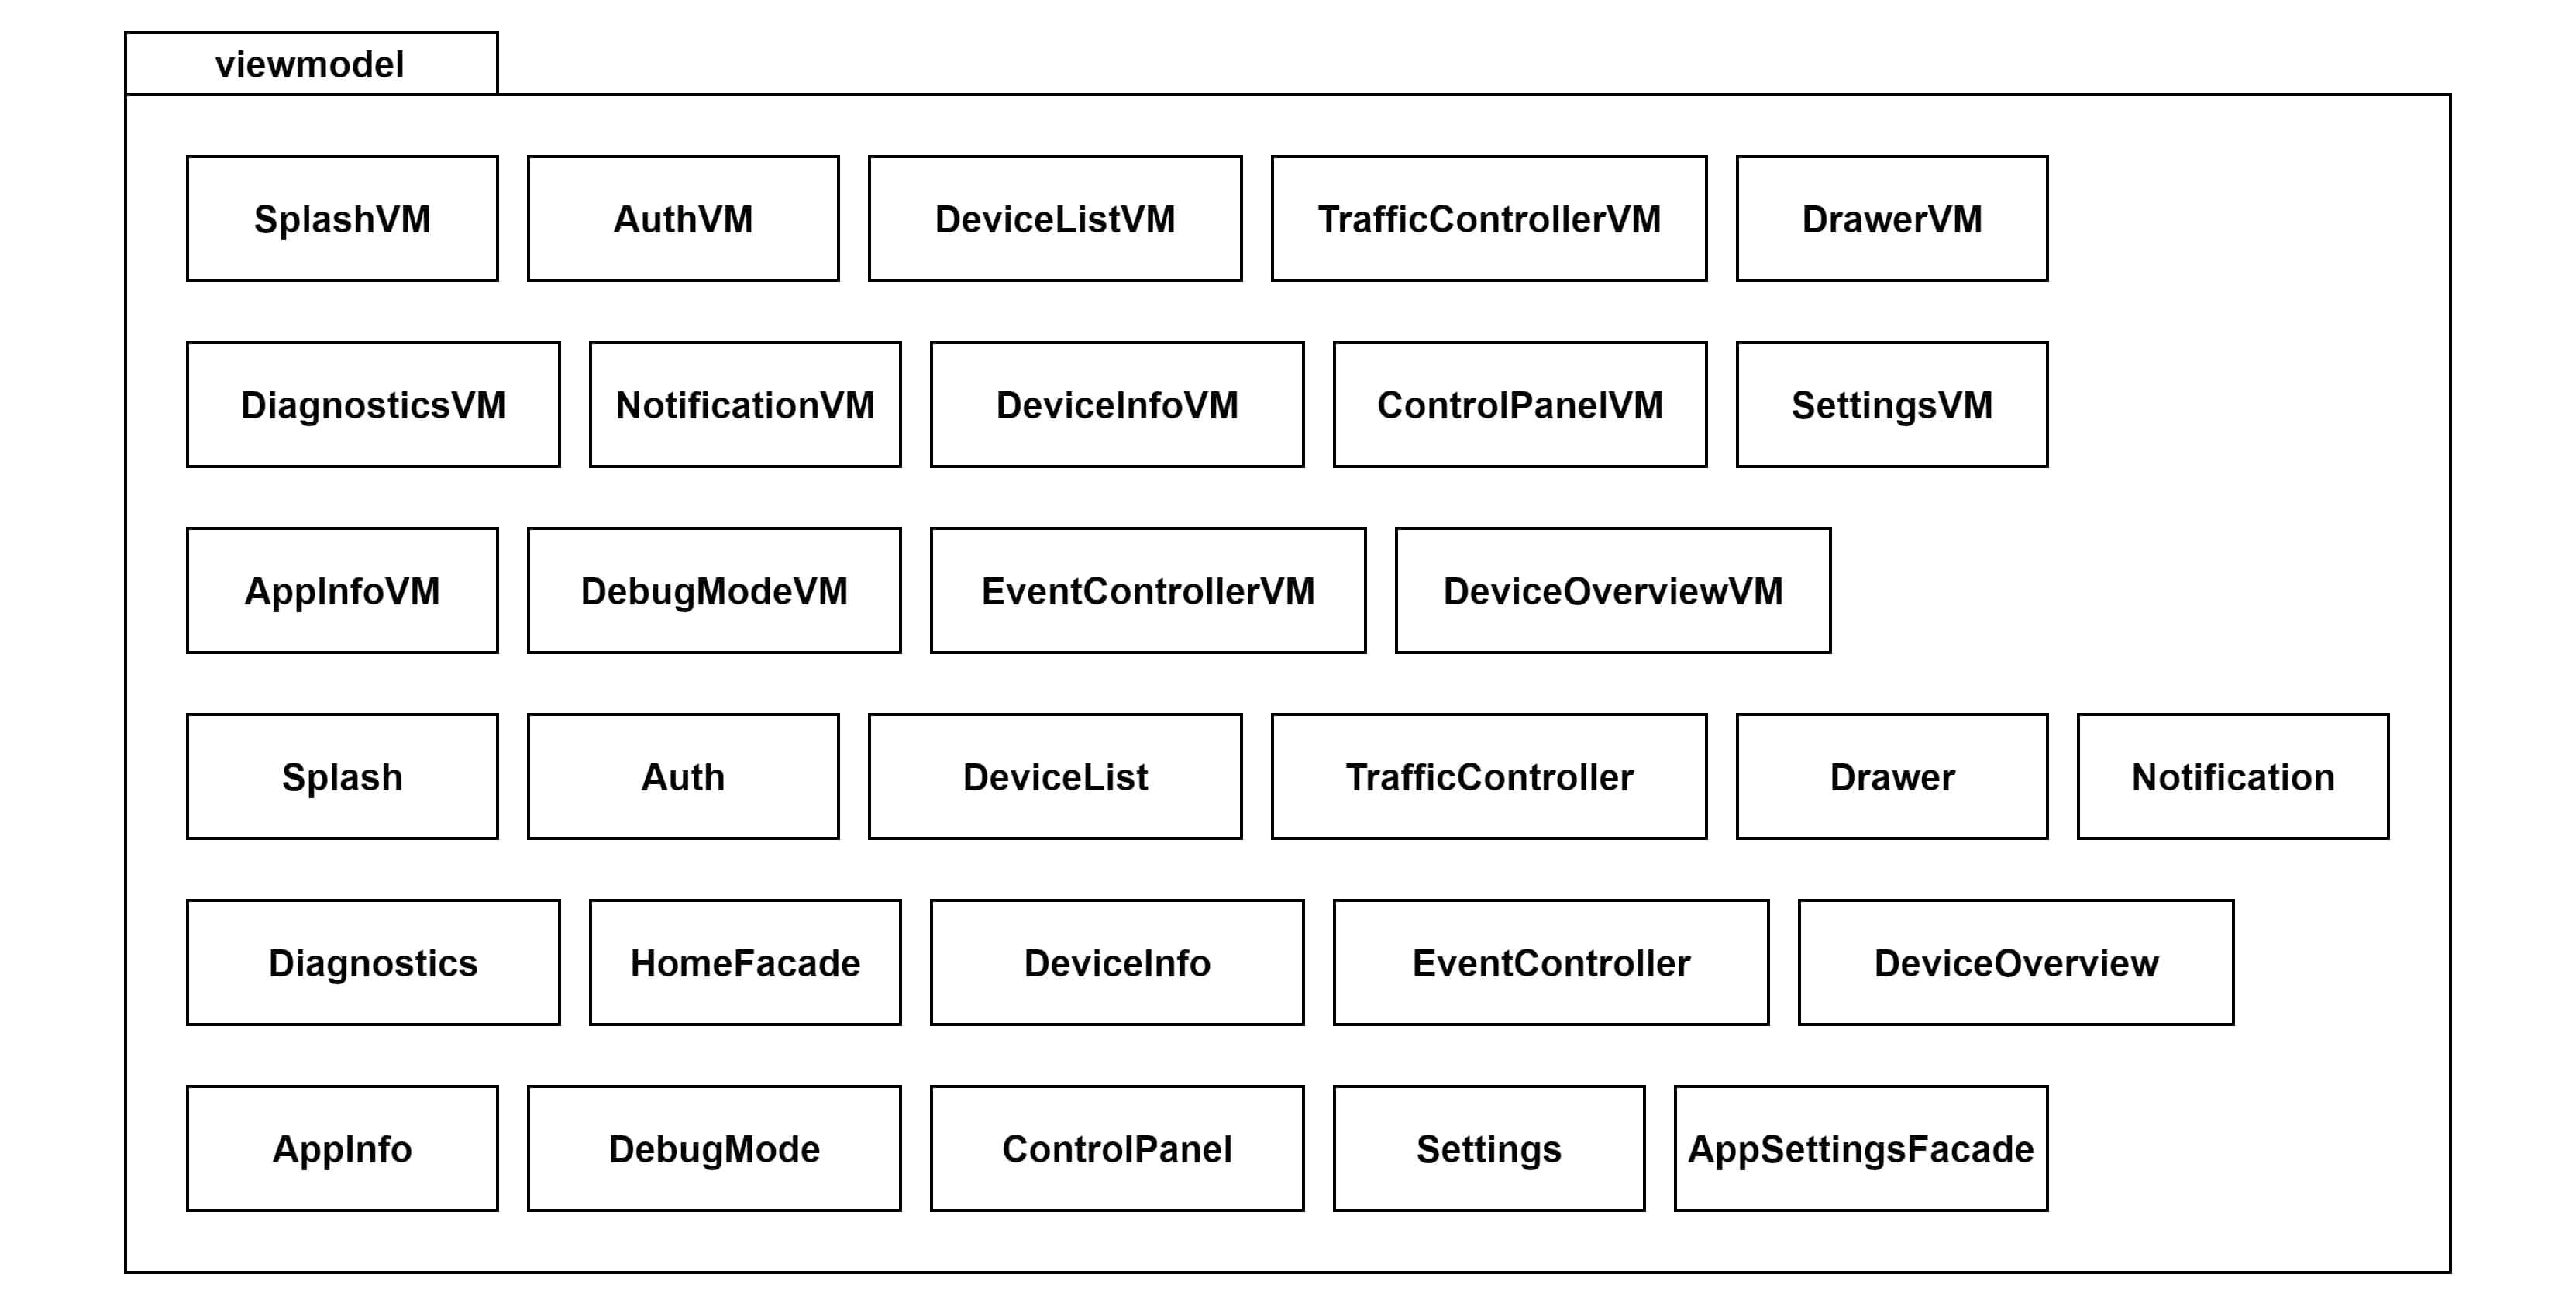
\includegraphics[width=1.0\columnwidth]{capitolo-6/organizzazione-package/viewmodel} 
  \caption{Diagramma del package \texttt{it.tecsen.smacs.viewmodel}}
\end{figure}
In questo package vi sono tutte le classi che implementano i viewmodel (ossia i model per le view) che permettono alle classi del package \texttt{view} di mostrare agevolmente i dati a schermo.\\
Per ogni viewmodel esiste un'interfaccia\footnote{Da qui in avanti in questa sezione, quando si utilizza il termine "interfaccia", si intende una classe astratta con tutti metodi astratti. Viene usato quindi il significato tipico di Java e non quello di Dart.} (tutte le classi che terminano con VM) e un'implementazione (le altre rimanenti).\\
Le classi \texttt{HomeFacade} e \texttt{AppSettingsFacade} non sono implementazioni di interfacce. Entrambi, come suggerisce il loro nome (\emph{facade}), sono classi che implementano l'omonimo \gls{designpatterng} per raggruppare funzionalità comuni necessarie alle classi del package \texttt{view}.
Il primo implementa funzionalità comuni per \texttt{SplashView} e \texttt{AuthView}. Il secondo contiene metodi e proprietà per la gestione delle impostazioni dell'applicazione, tra cui la presenza o meno di notifiche, lo stato del task in background e la durata del suo timeout di accensione.\\
Ogni interfaccia di questo package viene usata da una sola classe del package \texttt{view}, e queste non hanno accesso all'implementazione concreta. I \emph{facade} vengono invece usati in più classi dello stesso package.
